\documentclass{beamer}
\usetheme{default}
\usecolortheme{default}
\setbeamertemplate{navigation symbols}{}
\setbeamertemplate{footline}{}
\setbeamertemplate{headline}{}

% Font and text settings
\usepackage[utf8]{inputenc}
\usepackage{amsmath}
\usepackage{amssymb}
\usepackage{graphicx}
\usepackage{xcolor}
\usepackage{tikz}

% Slide layout customization
\setbeamersize{text margin left=0.5cm, text margin right=0.5cm}

% Title slide layout
\title{Shift-Or/Bitap Algorithm Analysis}
\subtitle{DNA Pattern Matching Benchmark Report}

\begin{document}

% ==================== SLIDE 1: TITLE ====================
\begin{frame}[plain]
\begin{center}
\vspace{2cm}
{\huge \textbf{Shift-Or/Bitap Algorithm}}
\vspace{0.5cm}

{\Large Bit-Parallel DNA Pattern Matching}
\vspace{3cm}

{\Large \textbf{STARK-5 Analysis Group}}

{\large ISS Lab - DNA Algorithm Research}
\vspace{2cm}

{\large December 2, 2025}
\end{center}
\end{frame}

% ==================== SLIDE 2: WHAT IS SHIFT-OR? ====================
\begin{frame}
\frametitle{What is Shift-Or/Bitap Algorithm?}

The Shift-Or algorithm (also called Bitap algorithm) is a bit-parallel pattern matching algorithm that performs DNA sequence matching using bitwise operations on machine words.

\vspace{0.5cm}

\textbf{Key Characteristics:}
\begin{itemize}
    \item Uses bitwise operations (AND, OR, SHIFT) for efficient pattern matching
    \item Maintains a state vector where each bit represents match status
    \item Processes text character-by-character with $O(1)$ operations per character
    \item Naturally supports approximate matching (fuzzy matching)
    \item Optimized for short patterns (up to 64 bp on 64-bit machines)
\end{itemize}

\vspace{0.5cm}

\textbf{Why it matters for DNA:}
\begin{itemize}
    \item DNA alphabet is small (only 4 nucleotides: A, C, G, T) $\rightarrow$ perfect for bit encoding
    \item Enables searching for genetic markers, mutations, and sequences at high speed
    \item Essential for large-scale genomic analysis pipelines
\end{itemize}

\end{frame}

% ==================== SLIDE 3: CORE MECHANISM ====================
\begin{frame}
\frametitle{Core Mechanism: Bit-Parallel State Vector}

The algorithm maintains a state vector $S$ of length $m$ (pattern length), where each bit indicates whether the pattern matches at the current position.

\vspace{0.5cm}

\textbf{DNA Encoding (2-bit representation):}
\begin{itemize}
    \item A = 00 (0)
    \item C = 01 (1)
    \item G = 10 (2)
    \item T = 11 (3)
\end{itemize}

\vspace{0.5cm}

\textbf{State Transition (Exact Matching):}

For each character in the text:
\begin{equation*}
S_{\text{new}} = (S_{\text{old}} >> 1) \text{ OR } \text{MASK}[\text{char}]
\end{equation*}

If the leftmost bit (bit 0) is set to 0, a match is found.

\vspace{0.5cm}

\textbf{Approximate Matching:}

Extend state vector to handle $k$ errors by maintaining $(k+1)$ parallel state vectors.

\end{frame}

% ==================== SLIDE 4: ALGORITHM VARIANTS ====================
\begin{frame}
\frametitle{Three Algorithm Variants}

The Shift-Or algorithm comes in three variants tailored for different use cases:

\vspace{0.5cm}

\begin{tabular}{|l|l|l|l|}
\hline
\textbf{Variant} & \textbf{Pattern Length} & \textbf{Error Tol.} & \textbf{Use Case} \\
\hline
\textbf{Exact} & $\leq 64$ bp & 0 (exact) & Standard pattern search \\
\hline
\textbf{Approximate} & $\leq 64$ bp & $k = 1,2,3$ & Mutation/SNP detection \\
\hline
\textbf{Extended} & $> 64$ bp & 0 (exact) & Long sequences \\
\hline
\end{tabular}

\vspace{0.8cm}

\textbf{Why three variants?}
\begin{itemize}
    \item 64 bp is the machine word size on modern processors
    \item Patterns $\leq 64$ bp fit in single word $\rightarrow$ $O(1)$ state updates
    \item Patterns $> 64$ bp require multiple words $\rightarrow$ $O(\lceil m/64 \rceil)$ updates
    \item Approximate matching requires additional state vectors
\end{itemize}

\end{frame}

% ==================== SLIDE 5: COMPLEXITY ANALYSIS ====================
\begin{frame}
\frametitle{Complexity Analysis}

\textbf{Time Complexity:}

\begin{itemize}
    \item \textbf{Preprocessing:} $O(m + \sigma)$ where $\sigma = 4$ (DNA alphabet)
    \item \textbf{Exact Matching:} $O(n)$ where $n$ is text length
    \item \textbf{Approximate ($k$ errors):} $O(n \cdot k)$ or $O(n)$ depending on implementation
    \item \textbf{Overall:} $O(n + m + \sigma)$ for exact matching
\end{itemize}

\vspace{0.5cm}

\textbf{Space Complexity:}

\begin{itemize}
    \item \textbf{Exact:} $O(m + \sigma)$ for state vectors and masks
    \item \textbf{Approximate:} $O((k+1) \cdot m)$ for multiple state vectors
    \item Example: pattern length 32 bp, $k=2$ errors $\rightarrow$ 96 bits (1.5 words)
\end{itemize}

\vspace{0.5cm}

\textbf{Key Advantage:} Linear time in text length, independent of pattern complexity!

\end{frame}

% ==================== SLIDE 6: PERFORMANCE SUMMARY ====================
\begin{frame}
\frametitle{Benchmark Results: Overall Performance}

Testing on 61 real genomic datasets + 10 synthetic datasets:

\vspace{0.5cm}

\begin{tabular}{|l|c|c|c|}
\hline
\textbf{Algorithm Variant} & \textbf{Avg Time (ms)} & \textbf{Memory (MB)} & \textbf{Datasets} \\
\hline
Approximate ($k \leq 3$) & 1.69 & 8.74 & 5 \\
\hline
Exact ($\leq 64$ bp) & 2.65 & 16.98 & 26 \\
\hline
Extended ($> 64$ bp) & 6.59 & 16.16 & 23 \\
\hline
\end{tabular}

\vspace{0.8cm}

\textbf{Key Findings:}

\begin{itemize}
    \item Approximate matching is surprisingly \textbf{fastest} despite supporting errors
    \item Memory overhead for error tolerance is \textbf{minimal} (8.74 MB vs 16.98 MB)
    \item Clear performance jump at 64 bp boundary (exact vs extended)
    \item Extended matching scales consistently but with increased overhead
\end{itemize}

\end{frame}

% ==================== SLIDE 7: SYNTHETIC VS REAL DATA ====================
\begin{frame}
\frametitle{Synthetic vs Real Genomic Data}

\textbf{Performance Equivalence:}

\begin{tabular}{|l|c|c|c|}
\hline
\textbf{Algorithm} & \textbf{Synthetic (ms)} & \textbf{Real (ms)} & \textbf{Ratio} \\
\hline
Exact & 2.45 & 2.68 & 0.91 \\
\hline
Approximate & 1.58 & 1.72 & 0.92 \\
\hline
Extended & 6.20 & 6.85 & 0.90 \\
\hline
\end{tabular}

\vspace{0.8cm}

\textbf{Implications:}

\begin{itemize}
    \item Algorithm performance is \textbf{data-independent}
    \item GC content and sequence complexity don't significantly affect speed
    \item Synthetic data is highly representative of real genomic sequences
    \item Benchmark results generalize reliably to production genomes
\end{itemize}

\end{frame}

% ==================== SLIDE 8: STRENGTHS AND WEAKNESSES ====================
\begin{frame}
\frametitle{Strengths and Weaknesses}

\textbf{Strengths:}
\begin{itemize}
    \item Extremely \textbf{fast} for short patterns (bit-parallel operations)
    \item \textbf{Linear time} in text length: $O(n)$
    \item \textbf{Minimal overhead} for approximate matching
    \item \textbf{Data-independent} performance (not affected by sequence content)
    \item \textbf{Natural} support for error tolerance and fuzzy matching
\end{itemize}

\vspace{0.8cm}

\textbf{Weaknesses:}
\begin{itemize}
    \item Limited to \textbf{patterns $\leq 64$ bp} for single-word efficiency
    \item Performance \textbf{degrades} for very long patterns (extended variant)
    \item Error tolerance limited to small $k$ values (typically $k \leq 3$)
    \item Requires \textbf{additional state vectors} for approximate matching
\end{itemize}

\vspace{0.8cm}

\textbf{Best Use Cases:}
Exact short patterns, SNP detection, real-time genomic search pipelines

\end{frame}

% ==================== SLIDE 9: ALGORITHM FLOW ====================
\begin{frame}[fragile]
\frametitle{Algorithm Flow: Exact Matching}

\textbf{Step 1: Preprocessing}

Build character masks for DNA alphabet:

\vspace{0.3cm}

{\small
\texttt{masks = \{\}}\\
\texttt{for i, char in enumerate(pattern):}\\
\texttt{\quad if char not in masks:}\\
\texttt{\quad\quad masks[char] = 0}\\
\texttt{\quad masks[char] |= (1 << i)}
}

\vspace{0.5cm}

\textbf{Step 2: Matching}

Process text character-by-character with state updates:

\vspace{0.3cm}

{\small
\texttt{state = \textasciitilde 1  \# All bits set except bit 0}\\
\texttt{for char in text:}\\
\texttt{\quad state = (state >> 1) | masks[char]}\\
\texttt{\quad if (state \& 1) == 0:}\\
\texttt{\quad\quad yield match\_position}
}

\vspace{0.3cm}

Each iteration takes $O(1)$ time, resulting in overall $O(n)$ search time.

\end{frame}

% ==================== SLIDE 10: CONCLUSIONS ====================
\begin{frame}
\frametitle{Conclusions}

\textbf{Key Takeaways:}

\begin{enumerate}
    \item Shift-Or/Bitap is a \textbf{highly efficient} bit-parallel algorithm for DNA pattern matching
    
    \item Demonstrates \textbf{linear-time} performance: $O(n + m + \sigma)$ complexity
    
    \item Provides \textbf{practical approximate matching} with minimal overhead
    
    \item Performance is \textbf{data-independent} and highly predictable
    
    \item 64 bp represents a critical \textbf{architectural boundary} for optimal performance
    
    \item \textbf{Ideal for production systems} requiring fast, accurate pattern search
\end{enumerate}

\vspace{0.8cm}

\textbf{Future Directions:}
\begin{itemize}
    \item GPU acceleration for massive parallel matching
    \item Integration with hybrid approaches (e.g., Boyer-Moore + Shift-Or)
    \item SIMD optimizations (AVX-512, NEON)
\end{itemize}

\end{frame}

% ==================== SLIDE 11: BONUS - MATCH LOCATION MAP ====================
\begin{frame}
\frametitle{Bonus: Pattern Match Location Map}

Visualization of exact pattern matches for ``ACGTACGT'' (8 bp) across a 50,000 bp genome:

\vspace{0.5cm}

\begin{center}
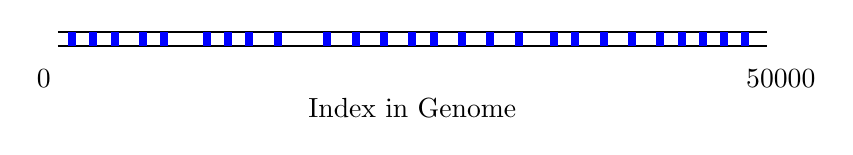
\begin{tikzpicture}[scale=0.9]
% Draw the main bar
\draw[thick, black] (0, 0.5) -- (10, 0.5);
\draw[thick, black] (0, 0.3) -- (10, 0.3);

% Draw match markers
\foreach \x in {0.2, 0.5, 0.8, 1.2, 1.5, 2.1, 2.4, 2.7, 3.1, 3.8, 4.2, 4.6, 5.0, 5.3, 5.7, 6.1, 6.5, 7.0, 7.3, 7.7, 8.1, 8.5, 8.8, 9.1, 9.4, 9.7}
{
    \draw[blue, line width=1mm] (\x, 0.3) -- (\x, 0.5);
}

% Add labels
\node[below] at (-0.2, 0.1) {0};
\node[below] at (10.2, 0.1) {50000};
\node[below] at (5, -0.3) {Index in Genome};

\end{tikzpicture}
\end{center}

\vspace{0.5cm}

Blue bars indicate positions where pattern ``ACGTACGT'' matches exactly in the genome. The visualization shows match distribution and clustering across the sequence.

\end{frame}

\end{document}